\documentclass{memoir}

\usepackage{import}
\import{../}{gov-style}
\addbibresource{../thesis.bib}

\begin{document}
\begin{refsegment}
\epigraph{``Hang the code, and hang the rules! They're more like guidelines anyway.''}{---\textup{Elizabeth Swan}}

\section{The rules of the game}
\subsection{A diplomatic parking ticket}
At the core of each chapter in this thesis is an argument about how states cooperate to apply the norms of espionage to emerging technology. In order for those arguments to make sense, though, it is first necessary to define exactly what those norms are and what it means to apply them to other areas of intelligence. That task is more difficult than it might seem.

The diplomatic protocol for espionage is not especially complicated. Most states maintain intelligence services---both civilian and military---whose job it is to collect information on other states, in order to better inform policy decisions. When one state uncovers the intelligence operation of another, both parties are aware that they are each equally guilty of espionage, regardless of which one happened to get caught at the moment. The two states will then engage in a familiar diplomatic tango: a public denunciation, an indignant denial, and possibly a prosecution or embassy expulsion. Even after having a particularly damaging operation uncovered---an agent deep within the adversary's government, for instance---the worst that is likely to happen is the expulsion of intelligence officers working in the embassy under diplomatic cover. Unlike many other aspects of international relations, the consequences almost never extend to another aspect of the relationship between those two states.

Losing embassy staffers who were identified---likely correctly---as intelligence officers is a legitimate consequence. It guts the embassy's operational presence and can have a lasting impact on that state's intelligence gathering ability in that nation for years to come.\footcite{macintyre_spy_2018} But expelling diplomats is also the worst-case consequence, and it has all the deterrent effect of a parking ticket. While states will go to great lengths to prevent espionage, at no point will they punish another state for trying. There will be no economic sanctions, linkage to other diplomatic issues, or significant change in the overall strategy of the intelligence service that was exposed. Like with a parking ticket, you simply pay the fine and you're free to drive again; the benefit gained from fare-dodging 50 times is well worth the price of getting caught once.\footnote{This thesis does not endorse violating municipal parking laws---it just makes the case that doing so absolutely pays off in the long run. Especially in Miami.}

% Moscow rules?

% Occasionally, a state will overstep the customary bounds, and in those cases the consequences are extended just enough to make it clear that this particular action is not within ``the rules of the game.'' This still happens today, most recently with the Russian poisoning of retired spy Sergei Skripal, who had been previously traded.Actions that overstep the boundaries also often take the form of covert operations, such as funding dissidents, enabling a coup, or disseminating propaganda.

% When an embassy staffer is outed as a spy by the host nation, that staffer is still subject to the customary protection of diplomatic immunity. The worst that can happen to them is to be declared \emph{persona non-grata} along with a handful of their colleagues and expelled from the country for ``activities incompatible with their diplomatic status.'' If the spy is not a diplomat, they will be tried and held captive (or killed), and if they are lucky they might get traded. Typically no further penalties are applied to the state that sent them.

In order to receive that minimized set of consequences, an operation must be within the bounds of what both states consider to be traditional espionage. This is difficult part: defining what constitutes traditional espionage. Supposedly, those bounds are defined by an internal morality that intelligence professionals call the ``rules of the game.'' When states impose harsher penalties, they often justify it by saying that they are punishing an operation that did not abide by the rules. For instance, the recent poisoning of Sergei Skripal, allegedly by Russian intelligence, was widely described a violation of the rules.\footcite{masters_has_2018} Assassinations are obviously off-limits, especially against former spies who have been traded to safety, and the US and the EU have issued multiple rounds of sanctions in response.\footcite{reuters_e.u._2019} Assassinations are also rare, though, and more often than not, an intelligence operation is understood by both parties to have been routine espionage, and the consequences are minimized accordingly.

As you might expect, these rules are not written down in a treaty. States are mostly unwilling to discuss how they collect intelligence, so they have few opportunities to definitively state what kinds of espionage are out of bounds.  The phrase ``rules of the game'' is barely more than a clich\'e, invoked casually by public officials, newspaper articles, and spy novels. Intelligence officers are doubtless sincere in their belief that espionage has a code, but the history of espionage suggests that the code is flexible, driven mostly by what intelligence agencies think they can get away with.

The rules of espionage elide definition because they do not exist, but they are important nonetheless, because they describe the unscientific process by which policymakers and intelligence agencies decide what types of operations are considered traditional---based on gut instinct and their experience with the field. Some operations just \emph{feel} like standard espionage. Take, for instance, the arrest of Adolf Tolkachev.  For six years, he ``provided plans, specifications and test results on existing and planned Soviet aircraft and missiles,'' until he was caught in 1985. The information that Tolkachev provided was a major coup for American intelligence. According to the CIA, he is considered by some intelligence historians to have been ``the greatest spy since Penkovsky.''\footcite{cia_look_2008} A \emph{New York Times} retrospective on intelligence, entitled ``Rules of Espionage: Got Caught? You Lose Players,'' describes his arrest like this:

\begin{quote}
At the end of one the most important spy operations run by the CIA against the Soviets during the cold war, for example, the Soviet scientist Adolf Tolkachev was detained in 1985. After Mr. Tolkachev's arrest and interrogation, the KGB lured a CIA officer, Paul Stombaugh, to what he believed was a meeting with Mr. Tolkachev. When Mr. Stombaugh arrived at the meeting site, the K.G.B. arrested him. He was quickly released; the sole purpose of the KGB ambush had been to out an American and briefly weaken the CIA's operations in Moscow.\footcite{risen_rules_2001}
\end{quote}
A year later, the Russian state news announced that they had executed Tolkachev for high treason, but the CIA, which facilitated his treason, suffered little more than small indignity of an expelled officer. Tolkachev's crime, while highly damaging to the Soviet Union, easily abided by what anyone with a passing understanding of intelligence would consider to be the rules of the game---he recorded information that he observed and passed it on to a foreign intelligence service.

No one can agree on exactly what activities the rules of the game prohibit, but copying documents and photographing machinery are clearly not among them. For this thesis, I am not interested in cases that test the limits of espionage---the assassination of former spies or the overthrow of democratically elected governments---but rather the cases that it would be impossible to dispute. Those are the cases that will tell us why the Director of the CIA said that hacking government records is ``fair game.'' For intelligence services introducing a new, powerful means of collecting intelligence, the goal is to make a novel activity seem in all other respects like something familiar. When the Chinese send a digital probe into the Office of Personnel Management, they don't want to push the limits; they want to play by the rules of the game.

% Norms, by definition, do not impose hard constraints on a state's ability to act---they suggest the contours of what a state will consider appropriate. To understand the norms of a particular field is to understand the range of options on the table and the likelihood that any given one will be chosen. Ideally, those norms are robust enough that it is possible to extrapolate a sort of policy rubric, in this case explaining how one state assesses an intelligence threat and then makes a response. If we understand the criteria by which the threat is evaluated, then we can explain why the government appears to consider only a limited range of responses to major cyberattacks, and predict which types of attack might elicit something stronger.

% The ambiguous status of espionage can cloak actions that were others be obviously impermissible. Rarely acknowledged by those in power, the diplomatic practices regarding espionage are quietly consistent and consistently quiet.

\subsection{Intelligence at the start of the Cold War}
% The norms governing espionage as old as nations themselves. An entire chapter of \emph{The Art of War} is devoted to the use of spies. ``Hence it is only the enlightened ruler and the wise general who will use the highest intelligence of the army for purposes of spying,'' counsels Sun Tzu. Thucydides mentions the role of ``informants'' within the city of Syracuse, who fed information to their Athenian besiegers.


The United States was the last major country in the world to establish an independent civilian intelligence service.\footcite[p.~35]{olson_fair_2006} Even after the success of the Office of Strategic Services (OSS) in WWII, Truman was still highly skeptical of a permanent civilian intelligence service. He reluctantly authorized the creations of the CIA in 1947, of which a third of the original employees were former OSS members.\footcite[p.~37]{olson_fair_2006} In an effort to ensure that the character of the intelligence service would be different from that of military intelligence, the initial command structure of Central Intelligence was dominated by the State Department.\footcite{troy_truman_1993}

Meanwhile, the Soviets exited World War II with perhaps the most formidable intelligence service on the planet. The KGB \emph{rezident}\footnote{The chief spy at an embassy. In the US, they would be known as a ``station chief.''} in London, Nikolai Rodin, boasted that no one could match the network of agents that Moscow had created there.\footcite[p.~151]{haslam_near_2015} And the Soviets had swiftly stolen one of America's most treasured wartime secrets, crucial information about the atomic bomb. When Truman first told Stalin that the Americans ``had a new weapon of unusual destructive force'' at the Potsdam conference in 1945, Stalin seemed ``neither surprised nor the least curious \textelp{} He did not, in fact, appear at all interested.''\footcite[p.~443]{mccullough_truman_1992}  Stalin's reaction was so off-putting that observers in the room wondered if he had even grasped the significance of what he'd been told. Apparently no one considered that Stalin simply already knew. Several highly paced Russian spies in the Manhattan project had already informed Stalin about the atomic bomb, and the Soviets had been running their own nuclear program since 1942.\footcite[p.~443]{mccullough_truman_1992}

Not only was the United States late to the game in setting up postwar a intelligence agency, it was also at a structural disadvantage when conducting HUMINT operations. Soviet Russia was a deeply paranoid and isolated state, and Western intelligence services faced a number of challenges running agents there. Every Western diplomat was placed under round-the-clock surveillance and significant travel restrictions, making it difficult to contact and turn potential agents. The USSR operated the world's most effective secret police, and Soviet citizens were told to be suspicious of foreigners.\footcite[p.~42]{richelson_american_1987} In 1943, the official State Department recommendation was simply to avoid undercover activity altogether.\footcite[p.~44]{richelson_american_1987} Compared to what the Soviet embassy in Washington was able to accomplish, the American embassy in Moscow was heavily handicapped.

This asymmetry raises an important question: if the system of undercover intelligence officers in each others' agencies clearly benefited the Soviet Union, then why did the United States continue to allow it? What preserves the norms of espionage when one side's relative gains are obvious? The asymmetry visible here is the norm, not the exception. The American disadvantage in HUMINT was the impetus for the cases examined in the following two chapters, where the United States acted as the norm entrepreneur, expanding intelligence norms to arenas where it had the advantage. Some calculus involving espionage norms kept the United States from blowing up the diplomatic protocol for human spies, and as you will see shortly, a similar calculus kept the Soviet Union from doing the same when the US began to deploy advanced technical means of gathering intelligence.

To explain how those norms held, the chapter is divided into three sections. In the first, I make it clear that at the start of the Cold War, espionage did not have any official protected status in the international legal regime. Not only did states have the right to respond to espionage however they liked, the legal norms regarding espionage were an open question---there was a plausible case to be made that espionage constituted a violation of territorial sovereignty. In the section after, I look briefly at the quantity of espionage that states dealt with during the Cold War and note how damaging some of these operations were; I use example of both American and Soviet espionage to demonstrate that the norm applies bidirectionally. Finally, I will propose a theoretical explanation for the consistent cooperation between states, from both a constructivist perspective and a defensive realist one.

% For espionage to have a specific set of associated consequences, it has to be expected that states will abide by those consequences, both when they catch an espionage operation and when they are caught.

% Therefore the examples in this chapter will demonstrate instances in which both the United States and the Soviet Union had to respond to damaging espionage operations conducted against them.


% it is important to note that regardless of which state is pushing to apply it, the norm has to cut both ways.

\section{Legality of espionage}
\subsection{An ambiguous wrong}
Espionage occupies a curious place in international law. It's clearly wrong, in the sense that treason and espionage are punished harshly under essentially every legal code. Many countries treat it as an unforgivable sin, where even falling under suspicion can lead to imprisonment, torture, and death. While the latter two punishments are sometimes criticized on human-rights grounds, no one disputes the right of a nation to punish those who work against them in service of a foreign power. The nation that sends a spy into a foreign country explicitly asks them to commit crimes on their behalf, and the spy risks paying the full price, all by themselves, if they are caught committing them.

The ``wrongness'' of violating a territorial boundary is extremely intuitive---the impermissibility of sending hostile military forces across a border line is foundational to the ontology of a nation-state and international legal conceptions of sovereignty.\footnote{I feel compelled to note that this is not the same as saying ``without borders with we have no nation'' in defense of restricting immigration, an argument which, regrettably, has some political currency today. Accommodating immigrants and refugees---stateless populations seeking to naturalize---is fundamentally different from being unable to repel invaders aligned with a hostile nation-state.} Early conceptions of spies considered them enemy combatants who were given none of the customary protections typically given to soldiers. The Hague Rules of 1907 and the Geneva Convention of 1949 both have guidelines outlining the limited permissibility of espionage during wartime, and the proper conduct for when a spy is apprehended.\footcite[p.~652]{beim_enforcing_2018} The former defines a spy this way:

\begin{quote}
A person can only be considered a spy when, acting clandestinely or on false pretenses, he obtains or endeavors to obtain information in the zone of operations of a belligerent, with the intention of communicating it to the hostile party. \\

Thus, soldiers not wearing a disguise who have penetrated into the zone of operations of the hostile army, for the purpose of obtaining information, are not considered spies. Similarly, the following are not considered spies: Soldiers and civilians, carrying out their mission openly, entrusted with the delivery of dispatches intended either for their own army or for the enemy's army. To this class belong likewise persons sent in balloons for the purpose of carrying dispatches and, generally, of maintaining communications between the different parts of an army or a territory. \\

A spy, taken in the act, shall not be punished without previous trial. \\

A spy who, after rejoining the army to which he belongs, is subsequently captured by the enemy, is treated as a prisoner of war, and incurs no responsibility for his previous acts of espionage (Articles 29-31).\footcite{noauthor_hague_1907} \\
\end{quote}
Though a bit dated, the Hague convention is routinely cited as a starting point for discussions about the legality of espionage, and as a description of an intelligence operative acting improperly in a foreign country, it works nicely. The problem with this definition is that its primary purpose is to distinguish between an enemy spy and an enemy soldier. Without a war there are no belligerents and no soldiers, so what is left with which to define a spy? In the United States---a country that has not issued a Declaration of War since 1942---it is not entirely clear under what circumstances the rules of wartime espionage would apply at all.\footcite{ncc_staff_when_2018}

% Valentino: It's interesting because this is very similar to the problem of terrorism. The US argues that because there is no formal war, terrorists are not combatants, and like spies, not subject to the protections offered to captured soldiers in times of war.

For our purposes, we can put aside the question of wartime espionage in the same way that University of Chicago Law Professor Quincy Wright does in a 1962 essay on this subject: if one takes the position that hostilities between the US and the USSR are sufficient to constitute a ``hot war,'' or that international law is always illusory, then the legality of espionage is irrelevant.\footcite[p.~8]{wright_espionage_1962} With the benefit of hindsight, neither of those propositions are true, so we can take it for granted that the US and the USSR were not at war, and the espionage that takes place between them is peacetime espionage.\footnote{I recognize that how to categorize the level of hostility in the Cold War is open to debate, as is the relevance of international law to states' actions. But however ``hot'' you think the Cold War really was, it clearly did not rise to the level where wartime rules about espionage would apply, and the only tool with which we have to evaluate the permissibility of peacetime espionage is international law.}

\subsection{Cold War debate about peacetime espionage}
The aforementioned essay by Professor Wright is part of a series of essays that to the best of my knowledge represent the first significant scholarly examinations of the legality of peacetime espionage. These \emph{Essays on Espionage and International Law} are interesting not only as a means to understand the evolution of scholarship historiographically, but also because they were published in 1962. At that time they were written, U-2 pilot Gary Powers was still in a Russian prison, and US and Soviet policymakers were still grappling with how to respond to the new reality of constant, frantic intelligence-gathering efforts. In the two essays of the collection that deal directly with HUMINT, Wright and Julius Stone, a professor of International Law at the University of Sydney, offer competing arguments for whether peacetime espionage---with or without territorial incursion---is itself an international delinquency.

Wright argued that peacetime espionage violates the principles of territorial integrity and political sovereignty. ``Any act by an agent of one state committed in another state's territory, contrary to the laws of the latter, constitutes intervention, provided those laws are not contrary to the state's international obligations.''\footcite[p.~13]{wright_espionage_1962} These are the same principles of territorial integrity that aerial reconnaissance violates, and as far as Wright was concerned, overflights were no different from human espionage. Both are unwanted incursions in space.

Since there are special wartime circumstances in which espionage is permitted, Wright allowed for the possibility that such circumstances might be present in peacetime. He individually analyzed the US government's defenses of the U-2 overflights as general justifications for all forms of espionage.\footcite[p.~17. A fun question to ask yourself is whether putting human spies and overflights in the same category elevates the severity of human intelligence or minimizes that of overflights. I think it actually does both, and Wright seemed to agree. An overflying plane is clearly capable of greater physical destruction but ``the difference should not be exaggerated. Although a reconnaissance airplane may carry bombs, a secret agent may plant a bomb and engage in various forms of sabotage.'' (p. 21) The general lack of concern that a spy plane might be carrying bombs is consistently surprising to me. Many of these flights were in retrofitted bombers, completely indistinguishable to enemies from their heavily-armed counterparts. Nonethless, both sides seem willing to treat reconnaissance flights as their own separate thing, and that protection applies to spies as well. As long as spies \emph{don't} engage in sabotage, the fact that they have the potential to do so is irrelevant.]{wright_espionage_1962} Most of these defenses came from the same general sentiment: everyone is doing it, and for our security we must as well. Wright was sympathetic, but after considering the different ways that states might spy on or interfere with each others' affairs, concluded that ``under present circumstances, it does not appear that a general rule justifying counter-intervention is expedient. Rather, action should be taken through the United Nations to terminate the original intervention.''\footcite[p.~22]{wright_espionage_1962} Paraphrased: none of this is justified, and it should be curbed through international judicial means.

% Valentino: The question of whether we would deal differently with acts of sabotage is interesting, since it has obvious parallels to the cyber debate. To my mind, though, the damage to national security that a well-placed spy or reconnaissance plane can do is far greater than anything but (maybe) a WMD.

Raising the issue of espionage in the United Nations is a plausible option but, in practice, most states dodge international law entirely by simply disowning their spies. This is how Wright described the status quo in 1962: ``Since the government responsible \textelp{} seldom acknowledges its responsibility but allows the agent, if caught, to be punished without protest, such incidents are not usually the subject of international discussion.''\footcite[p.~15. As an argument for not invoking international law, I acutally find this a bit silly. Just because a bank robber never flips on their co-conspirators does not mean those co-conspirators cannot be indicted for their role in committing the crime.]{wright_espionage_1962}

% Valentino: Question for Wright is really whether the state has the right to do MORE than just punish the captured spy. What is it allowed to do to punish the state that sent the spy. Can it launch a military attack and claim the right of territorial self-defense?

Professor Stone's view was that the illegal aspects of espionage are the ancillary territorial violations that sometimes make it possible, not the espionage itself. Where Wright saw the the disowning of spies as evidence of espionage's illegality, Stone saw it as a \emph{de facto} endorsement. ``Surely if espionage were a state delinquency in itself'' he writes, ``the aggrieved state would not always have been content to take such disclaimers at their face value.''\footcite[p.~33]{stone_legal_1962} Though Stone made a point to ``register an almost complete dissent from [Wright's] view'', they both arrived at similar conclusions regarding the practice of peacetime espionage.\footcite[p.~33]{stone_legal_1962} The vast majority of the time, states are going to deny that they were involved in espionage when their spies are caught, and the other state is going to let them. When it comes to prosecution ``it belongs to each state to define peacetime espionage, sedition, subversion, sabotage, incitement, and conspiracy as it sees fit.''\footcite[p.~4]{wright_espionage_1962} The spies are on their own.\footnote{Neither author addresses how spies can be subsequently traded if both sides reuse to acknowledge their original involvement. Gary Powers was exchanged for Rudolph Abel that same year.}

% I will actually go one step further than Stone here and argue that in some cases high-quality intelligence, even when obtained through deceit, is \emph{better} than the same information obtained though mutually reciprocated inspection channels. Assuming that the source is reliable, then you know that the adversary (or ally) from whom the intelligence was obtained did not want you to have it, and that lends the intelligence credibility. The paradox of espionage is that it has to be punishable, or it wouldn't be espionage.\footcite[p.~347]{demarest_espionage_1995}

In the case of espionage, states are not particularly concerned about whether or not their activities are delinquency under international law. The purpose of this debate is to illustrate that, over a decade into the Cold War, the legal status of peacetime espionage was far still from clear. Wright and Stone both offer reasonable interpretations of how espionage fits in to international law. An opportunistic state could have deployed a restrictionist explanation, like Wright's, as justification for cracking down on espionage; instead, they chose (consciously or unconsciously) to consistently interpret international law so as to allow it.

% Valentino: This is your point. But your argument is not that states don't think they are ``delinquencies'' under international law, but that they have chosen (conciously or unconciously) to interpret international law so as to allow it. The fact that Wright can make a seasonable argument that espionage should be illegal, shows that states had the flexibility with the law to go either way.

\subsection{Espionage controversies}
Generally speaking, civil society conditions us to think of intelligence operations as one of those things that every country \emph{just does}, legal or not. The average citizen has to hope that our government is using the appropriate discretion in choosing to undertake these missions that we know nothing about, and expect that they are defending against those same attempts by others. That nations will use their intelligence agencies to collect the state secrets of others is, in its barest form, a relatively noncontroversial premise. After all, intelligence agencies exist in plain sight.

That is not to say espionage in uncontroversial. The public level of comfort with the nature and scale of these secret activities naturally varies, especially in liberal democracies with a free press. Daniel Ellsberg's decision to release the Pentagon Papers in 1971 precipitated the first in a series of scandals that plagued the CIA during that decade---electoral interference in Chile, domestic spying on antiwar activists, and complicity in Watergate all contributed to widespread distrust of American intelligence operations.\footcite[p.~214-215]{andrew_missing_1984} In 1975-6, Jimmy Carter explicitly campaigned for president on a promise to curtail the independence and abuses of American intelligence agencies.\footcite[p.~217]{andrew_missing_1984} Ronald Reagan would later unseat Carter with a promise to restore those capabilities, only to later find himself embroiled in his own covert action scandal, when senior administration officials and the CIA were implicated in the Iran-Contra affair.

Even in the occasions when the American public demanded functional limits on policymakers' ability to conduct covert operations abroad, the basic premise that the US government should conduct espionage on other countries has always remained unquestioned. At the height of anti-CIA sentiment in the '70s, Congress passed the Hughes-Ryan Amendment, which was intended to restore the CIA's original conception as an agency for intelligence only.\footcite[p.~215]{andrew_missing_1984} The Amendment prohibits CIA funds from being used for any activities other than ``activities intended solely for obtaining necessary intelligence.'' Hughes-Ryan and the Intelligence Oversight Act of 1980 are the only major pieces of legislation that curtailed CIA independence for the entire Cold War, spanning 1947-1991.\footcite[p.~93-94]{cogan_covert_1993} Both reaffirm the basic necessity of maintaining a civilian intelligence service by contrasting ``good'' foreign intelligence gathering with ``bad'' covert action and interference.

% \subsection{Espionage in diplomacy}
% While not explicitly condoned, civilian and military intelligence agencies routinely facilitate espionage---against both enemies and allies---that is often in violation of the domestic law of the nation being spied upon. Explicitly encouraging foreign nationals to undermine the security of their own state would seem to be a violation of domestic sovereignty, but it is for various reasons a normalized practice, and one that is occasionally even acknowledged by people in power. That delicate balance---where espionage is clearly illegal but also expected, acknowledged, and accepted---is maintained by a retaliation structure that carefully preserves every state's right to attempt espionage themselves.

% This way this works is law enforcement agencies do everything possible to frustrate and discourage the act of espionage itself without discouraging the development of a market for the information that espionage provides. Employees and contractors that deal in high-level government secrets are carefully vetted. Counterintelligence officers engage in all kinds of expensive and time-consuming trickery to catch spies in the act. In most places, espionage is a capital crime, punishable by long prison sentences, torture, and in some cases, death. These measures all increase the price of intelligence, but they leave its buyers intact. As long as there are states willing to pay for confidential information, then there will always be someone desperate or disillusioned enough to provide it. States are not only aware of that fact, they rely on it, and limit the inter-state consequences for running a successful intelligence operation accordingly.

\section{Frequency of espionage}
\subsection{Categories of spies}
Human intelligence is a very broad category, and there are a lot of different types of spies. Depending on the nature of the spy's activities and the pretense under which they were operating, the offensiveness of their presence can vary dramatically, so we would expect that the diplomatic reaction might vary as well. With that in mind, what are the kinds of human intelligence operations that a state will be expected to respond to, and how have they responded to them in the past?

Broadly speaking, there are three types of spies that a state might uncover: a foreign national operating under diplomatic cover, a foreign national ``illegal,'' and one of its own citizens (generally working for the government or military) with access to useful information who agrees to operate as an agent for a foreign intelligence agency.\footnote{Terminology note: As the CIA defines it, a person working for their own country's intelligence service is an ``officer,'' and the foreign national working providing information is an ``agent.'' These could possibly be different for other intelligence services, but they seem to be pretty consistent.(\cite{cia_insider_2019})} That is not to say that every person who works for a foreign government---even in secret---is by definition a spy. Many activities that fall short of espionage can still serve the purposes of a foreign power. Russia, for instance, regularly funded leftist magazines and news outlets in Western countries, and kept tabs on socialist or communist sympathizers who might be predisposed to provide them with information or assistance. Those sympathizers, who might have knowingly socialized with and taken money from Soviet agents, are still not necessarily spies.

There are also three main ways that a spy's career can end: they can retire, they can defect, or they can get caught. Since retirement is a non-issue diplomatically, the latter two endings, defection or capture, are where the consequences come into play. Not all defections are created equal. If a civilian or spy walks into an embassy and publicly switches allegiances, there isn't much that either side can do about it. Such was the case with Soviet Captain Nikolay Khokhlov, who in February 1954, while on a mission to assassinate an official in a Russian refugee organization, instead revealed the plot to his target and turned himself in to American agents in West Germany, defecting with his wife.\footcite[Captain Khoklov repeatedly emphasized at the press conference that his decision to defect was inspired by his wife Yanina, who told him that ``she would never permit their child to have an assasin as a father.'']{handler_another_1954} In addition to bringing along his two co-conspirators, Khokhlov helped the United States identify a number of other Soviet agents.

The Khokhlov incident was embarrassing for the USSR, but their diplomatic options were limited. In theory, they could have demanded that the Americans return the officer, since he had committed high treason against their country. The United States would likely have refused, and then incident could have escalated further. But because the crime that Khokhlov committed was revealing a Soviet plot, not to mention an especially offensive one (assassinations are acceptable pretty much nowhere), any noise made by the Soviets to get their man back would have brought more attention to the original plot. Their diplomatic recourse was limited---the Soviets were in the wrong, and the US simply accepted information that was freely given to them. Instead, the Soviets attempted to assassinate their former assassin. Khokhlov survived the attempted poisoning and lived the rest of his life as an academic in California. He was pardoned by Boris Yeltsin in 1992 and passed away in 2007.\footcite[p.~57]{mickolus_counterintelligence_2015}

A defection, as Kohklov's case illustrates, carries no consequences for the state that receives the defector. There just isn't anything to blame them for. They didn't conspire to undermine the another state in violation of their domestic law, they were offered a gift and they took it. If anything, such a defection carries more potential consequences for the defector's former nation, because the defector is likely to reveal information about their intelligence operations, leading to the arrest of active agents. Defections are often a crucial source of counterintelligence.

So what kinds of spying cases could potentially have associated repercussions? The ones where a state continually facilitates violations of domestic espionage law. There are two main cases in which this could be the case. The first is if the host nation discovers that embassy staffers are undercover intelligence officers. According to Robert Booth, former counterintelligence officer for the State Department, it is very easy for counterintelligence to figure out which diplomats are undercover spies, through a number of telltale signs about the diplomat's background.\footcite{booth_personal_2019} This happens all the time, and in most cases, the host state will choose to simply monitor the officer, rather than expel them. That way, they can their movements and potentially even uncover other operations.\footcite{booth_personal_2019} When diplomats are expelled, it is often as collateral damage for another incident in which they may or may not have taken part.

\subsection{Quantity of captured spies}
For the aggregate analysis in this chapter, I will focus on the category of spy that has the most potential for diplomatic incident---someone who passes important information to a foreign intelligence service without the knowledge of the country providing the information. The diplomatic provocation here is that one state purposefully enabled the violation of the other's domestic laws, and did so in service of obtaining information that could potentially be highly damaging to their national security. These spies are often citizens who either hold positions which grant them access to privileged information, or they work adjacent to people who do. Often these are citizens of the nation being spies upon, but occasionally they are illegals, deep-cover spies with fabricated backgrounds who perform limited work in order to maintain their cover.

Human Intelligence (HUNINT) presents a clear example of the international norm that legitimizes espionage without authorizing it. Over the course of the Cold War both sides uncovered quite a few spies, and most of their cases were handled without any diplomatic consequences whatsoever. Even the most damaging, newsworthy, spectacle cases had no consequences beyond some barbed words and diplomatic expulsions. Likewise, the state conducting the espionage was not discouraged from continuing to do so even in situations where critical information about national security was compromised. To demonstrate this a case-based approach is necessary, but so is an aggregate analysis of the quantity of espionage taking place during the Cold War.

% In the aerial espionage chapter, I took the approach of examining a particularly tense period in the early Cold War during which aerial reconnaissance played a crucial role in the American ability to asses the military capabilities of their Soviet adversaries. As satellites soon rendered most of these missions obsolete, the time frame in which these flights were a significant diplomatic issue is limited to a period of about 15 years. Argumentatively, it was feasible to discuss each of those 13 flights shot down by the USSR---along with a few related aerial incidents---and subsequently argue that all of their diplomatic responses fit within the confines of the limit that I am establishing. With HUMINT the quantity of potential incidents is substantially greater. Aerial reconnaissance eventually took a backseat to satellites and other forms of gathering SIGINT, but using spies to gather intelligence remained relevant throughout the entirety of the Cold War. With the space I have, I cannot write about every single unmasked spy and assess the diplomatic consequences of their exposure---there are simply too many.

To do so, I examine the list of the spy cases that the United States dealt with during the Cold War and talk about how they were handled in the aggregate. The task of assembling that list is difficult. Federal criminal prosecutions are notoriously difficult to generate data for, even without the added secrecy of espionage. Even though the information is not listed anywhere officially, there are a finite number of people who have been publicly accused of spying against the United States, and researchers have been able to compile a comprehensive database of domestic spy cases. The two best data-based approaches to American espionage history that I have found are Edward Mickoulous' \emph{The Counter-Intelligence Chronology} and the Defense Personnel Security Research Center's (PERSEREC) \emph{Espionage against the United States by American Citizens 1947-2001} report. PERSEREC also maintains a database of ``Espionage and other Compromises of National Security'' from 1975 to present day.

\emph{The Counter-Intelligence Chronology} is a book-length timeline of significant moments in the intelligence history of the United States, including espionage both for and against the United States. It also contains an accompanying appendix with a list of alleged American spies, and a year associated with each name.\footcite[p.~173]{mickolus_counterintelligence_2015} I digitized this list and reproduced it in the Appendix section of this chapter. The criteria for inclusion in this list is to be an American citizen or long-term resident who was investigated (and in some cases arrested, charged, convicted, or cleared) for espionage or who defected to foreign intelligence services. Because each case is different, the year included with each name does not precisely correlate with any one thing. It could be an arrest, or the date they were first investigated, or something else. Julius and Ethel Rosenberg are both listed as July 17, 1950, even though that is the date of Julius' arrest---Ethel was arrested a month later. It is best to think of the date as the time when the spy fell under public suspicion.

For our purposes, the date works as a decent proxy for the moment when that particular case could have become a diplomatic incident. I aggregated the spy cases by decade, the results of which you can see in Figure \ref{decade_spies}. Most (but not all) of these incidents have an entry associated with them in the main \emph{Chronology} timeline. I will describe what those entries tend to look like in a moment, but for the moment just know that each incident represents someone who either was tried for espionage against the United States on behalf of the USSR, or would have been had they not escaped.\footnote{The United States does not try defendants \emph{in absentia}, a principle that has held since the Supreme Court's 1884 ruling in Hopt v. Utah, and codified by the Federal Rules of Criminal Procedure in 1946. (\cite{noauthor_rule_1946-1}) The Russians have no such qualms, and have on multiple occasions prosecuted defectors after successfully fled. (\cite{traynor_trial_2002})}

\begin{figure}[ht]
  \centering
  % Created by tikzDevice version 0.12 on 2019-03-10 18:28:25
% !TEX encoding = UTF-8 Unicode
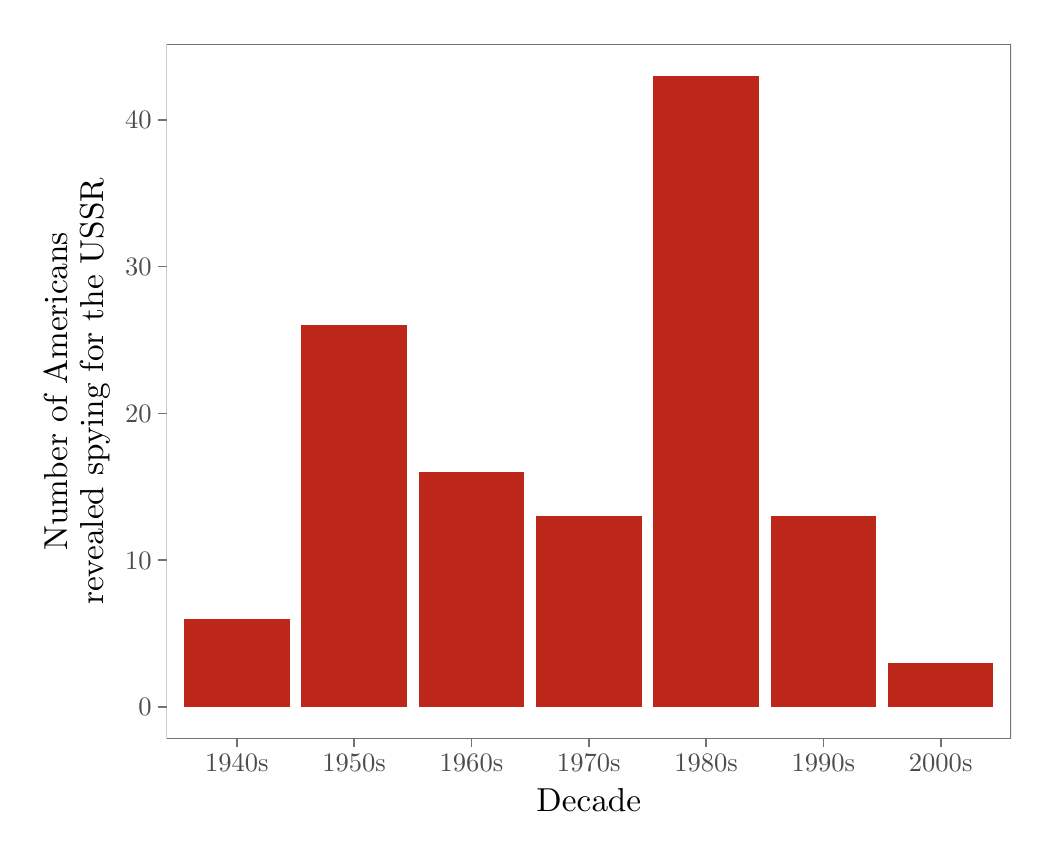
\begin{tikzpicture}[x=1pt,y=1pt]
\definecolor{fillColor}{RGB}{255,255,255}
\path[use as bounding box,fill=fillColor,fill opacity=0.00] (0,0) rectangle (361.35,289.08);
\begin{scope}
\path[clip] (  0.00,  0.00) rectangle (361.35,289.08);
\definecolor{drawColor}{RGB}{255,255,255}
\definecolor{fillColor}{RGB}{255,255,255}

\path[draw=drawColor,line width= 0.6pt,line join=round,line cap=round,fill=fillColor] (  0.00,  0.00) rectangle (361.35,289.08);
\end{scope}
\begin{scope}
\path[clip] ( 50.17, 32.28) rectangle (355.35,283.08);
\definecolor{fillColor}{RGB}{255,255,255}

\path[fill=fillColor] ( 50.17, 32.28) rectangle (355.35,283.08);
\definecolor{fillColor}{RGB}{188,39,26}

\path[fill=fillColor] ( 56.52, 43.68) rectangle ( 94.67, 75.49);

\path[fill=fillColor] ( 98.91, 43.68) rectangle (137.06,181.54);

\path[fill=fillColor] (141.30, 43.68) rectangle (179.45,128.51);

\path[fill=fillColor] (183.68, 43.68) rectangle (221.83,112.61);

\path[fill=fillColor] (226.07, 43.68) rectangle (264.22,271.68);

\path[fill=fillColor] (268.46, 43.68) rectangle (306.61,112.61);

\path[fill=fillColor] (310.84, 43.68) rectangle (348.99, 59.58);
\definecolor{drawColor}{gray}{0.45}

\path[draw=drawColor,line width= 0.6pt,line join=round,line cap=round] ( 50.17, 32.28) rectangle (355.35,283.08);
\end{scope}
\begin{scope}
\path[clip] (  0.00,  0.00) rectangle (361.35,289.08);
\definecolor{drawColor}{gray}{0.30}

\node[text=drawColor,anchor=base east,inner sep=0pt, outer sep=0pt, scale=  0.96] at ( 44.77, 40.37) {0};

\node[text=drawColor,anchor=base east,inner sep=0pt, outer sep=0pt, scale=  0.96] at ( 44.77, 93.39) {10};

\node[text=drawColor,anchor=base east,inner sep=0pt, outer sep=0pt, scale=  0.96] at ( 44.77,146.42) {20};

\node[text=drawColor,anchor=base east,inner sep=0pt, outer sep=0pt, scale=  0.96] at ( 44.77,199.44) {30};

\node[text=drawColor,anchor=base east,inner sep=0pt, outer sep=0pt, scale=  0.96] at ( 44.77,252.47) {40};
\end{scope}
\begin{scope}
\path[clip] (  0.00,  0.00) rectangle (361.35,289.08);
\definecolor{drawColor}{gray}{0.45}

\path[draw=drawColor,line width= 0.6pt,line join=round] ( 47.17, 43.68) --
	( 50.17, 43.68);

\path[draw=drawColor,line width= 0.6pt,line join=round] ( 47.17, 96.70) --
	( 50.17, 96.70);

\path[draw=drawColor,line width= 0.6pt,line join=round] ( 47.17,149.72) --
	( 50.17,149.72);

\path[draw=drawColor,line width= 0.6pt,line join=round] ( 47.17,202.75) --
	( 50.17,202.75);

\path[draw=drawColor,line width= 0.6pt,line join=round] ( 47.17,255.77) --
	( 50.17,255.77);
\end{scope}
\begin{scope}
\path[clip] (  0.00,  0.00) rectangle (361.35,289.08);
\definecolor{drawColor}{gray}{0.45}

\path[draw=drawColor,line width= 0.6pt,line join=round] ( 75.60, 29.28) --
	( 75.60, 32.28);

\path[draw=drawColor,line width= 0.6pt,line join=round] (117.98, 29.28) --
	(117.98, 32.28);

\path[draw=drawColor,line width= 0.6pt,line join=round] (160.37, 29.28) --
	(160.37, 32.28);

\path[draw=drawColor,line width= 0.6pt,line join=round] (202.76, 29.28) --
	(202.76, 32.28);

\path[draw=drawColor,line width= 0.6pt,line join=round] (245.14, 29.28) --
	(245.14, 32.28);

\path[draw=drawColor,line width= 0.6pt,line join=round] (287.53, 29.28) --
	(287.53, 32.28);

\path[draw=drawColor,line width= 0.6pt,line join=round] (329.92, 29.28) --
	(329.92, 32.28);
\end{scope}
\begin{scope}
\path[clip] (  0.00,  0.00) rectangle (361.35,289.08);
\definecolor{drawColor}{gray}{0.30}

\node[text=drawColor,anchor=base,inner sep=0pt, outer sep=0pt, scale=  0.96] at ( 75.60, 20.26) {1940s};

\node[text=drawColor,anchor=base,inner sep=0pt, outer sep=0pt, scale=  0.96] at (117.98, 20.26) {1950s};

\node[text=drawColor,anchor=base,inner sep=0pt, outer sep=0pt, scale=  0.96] at (160.37, 20.26) {1960s};

\node[text=drawColor,anchor=base,inner sep=0pt, outer sep=0pt, scale=  0.96] at (202.76, 20.26) {1970s};

\node[text=drawColor,anchor=base,inner sep=0pt, outer sep=0pt, scale=  0.96] at (245.14, 20.26) {1980s};

\node[text=drawColor,anchor=base,inner sep=0pt, outer sep=0pt, scale=  0.96] at (287.53, 20.26) {1990s};

\node[text=drawColor,anchor=base,inner sep=0pt, outer sep=0pt, scale=  0.96] at (329.92, 20.26) {2000s};
\end{scope}
\begin{scope}
\path[clip] (  0.00,  0.00) rectangle (361.35,289.08);
\definecolor{drawColor}{RGB}{1,2,2}

\node[text=drawColor,anchor=base,inner sep=0pt, outer sep=0pt, scale=  1.20] at (202.76,  6.00) {Decade};
\end{scope}
\begin{scope}
\path[clip] (  0.00,  0.00) rectangle (361.35,289.08);
\definecolor{drawColor}{RGB}{1,2,2}

\node[text=drawColor,rotate= 90.00,anchor=base,inner sep=0pt, outer sep=0pt, scale=  1.20] at ( 14.26,157.68) {Number of Americans };

\node[text=drawColor,rotate= 90.00,anchor=base,inner sep=0pt, outer sep=0pt, scale=  1.20] at ( 27.22,157.68) {revealed spying for the USSR};
\end{scope}
\end{tikzpicture}

  \label{decade_spies}
  \caption{Number of Americans alleged to be spying for the USSR, by decade}
\end{figure}

The PERSEREC report is older, but because it is exclusively focused on cataloging espionage against the United States, it goes into some detail that the Mickoulous book leaves out. PERSERC, which sits within the Department of Defense, was actually founded in 1986 to provide policymakers and citizens with a database to conduct research on espionage.\footcite[p.~v]{herbig_espionage_2002} Though PERSERC is a government entity, the data provided is based entirely on open-source information. For their analysis of the prevalence of spies, they take a slightly different tact and count the number of spies known to be active during a given year; a spy will be counted each year that they are active, rather than how I aggregated them above where a spy will be counted exactly once, during the year in which they fall under suspicion. I reproduced the PERSERC active spies chart in Figure \ref{perserec_spies}. While not all of these spies were spies for the USSR, 56\% of them were, and if you add in spies for the other Soviet Bloc countries who could be relied upon to pass on their information to the USSR, that percentage jumps to 76\%.\footcite[p.~62-63. Herbig and Wiskoff use this method to estimate the amount of espionage undertaken on behalf of the USSR, directly or otherwise.]{herbig_espionage_2002}

\begin{figure}[ht]
  \centering
  % Created by tikzDevice version 0.12 on 2019-03-30 20:59:36
% !TEX encoding = UTF-8 Unicode
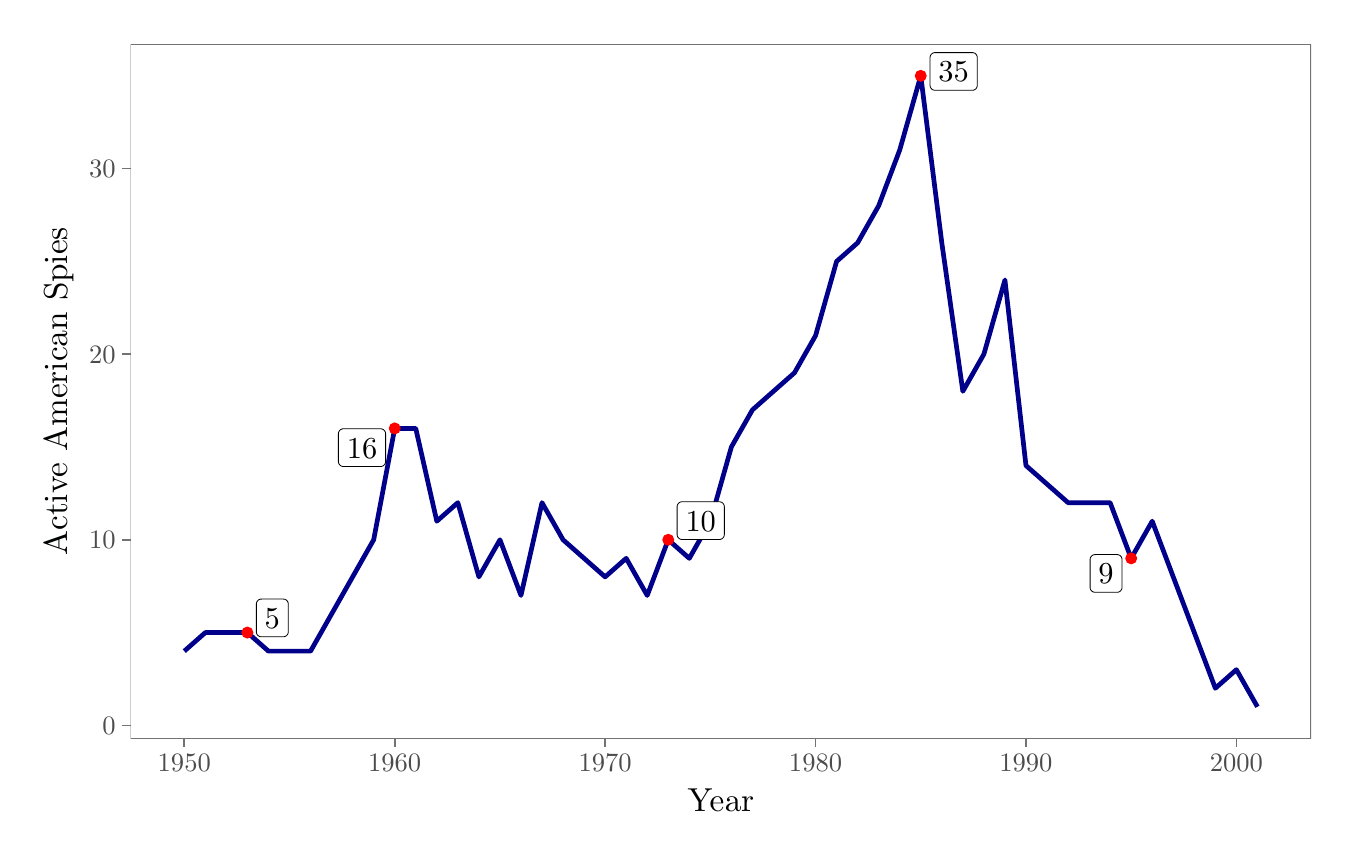
\begin{tikzpicture}[x=1pt,y=1pt]
\definecolor{fillColor}{RGB}{255,255,255}
\path[use as bounding box,fill=fillColor,fill opacity=0.00] (0,0) rectangle (469.75,289.08);
\begin{scope}
\path[clip] (  0.00,  0.00) rectangle (469.75,289.08);
\definecolor{drawColor}{RGB}{255,255,255}
\definecolor{fillColor}{RGB}{255,255,255}

\path[draw=drawColor,line width= 0.6pt,line join=round,line cap=round,fill=fillColor] (  0.00,  0.00) rectangle (469.76,289.08);
\end{scope}
\begin{scope}
\path[clip] ( 37.21, 32.28) rectangle (463.75,283.08);
\definecolor{fillColor}{RGB}{255,255,255}

\path[fill=fillColor] ( 37.21, 32.28) rectangle (463.75,283.08);
\definecolor{drawColor}{RGB}{0,0,139}

\path[draw=drawColor,line width= 1.7pt,line join=round] ( 56.59, 63.79) --
	( 64.20, 70.50) --
	( 71.80, 70.50) --
	( 79.40, 70.50) --
	( 87.01, 63.79) --
	( 94.61, 63.79) --
	(102.22, 63.79) --
	(109.82, 77.21) --
	(117.42, 90.62) --
	(125.03,104.03) --
	(132.63,144.27) --
	(140.23,144.27) --
	(147.84,110.74) --
	(155.44,117.44) --
	(163.04, 90.62) --
	(170.65,104.03) --
	(178.25, 83.91) --
	(185.85,117.44) --
	(193.46,104.03) --
	(201.06, 97.32) --
	(208.66, 90.62) --
	(216.27, 97.32) --
	(223.87, 83.91) --
	(231.47,104.03) --
	(239.08, 97.32) --
	(246.68,110.74) --
	(254.28,137.56) --
	(261.89,150.97) --
	(269.49,157.68) --
	(277.09,164.38) --
	(284.70,177.80) --
	(292.30,204.62) --
	(299.90,211.33) --
	(307.51,224.74) --
	(315.11,244.86) --
	(322.71,271.68) --
	(330.32,211.33) --
	(337.92,157.68) --
	(345.52,171.09) --
	(353.13,197.91) --
	(360.73,130.85) --
	(368.33,124.15) --
	(375.94,117.44) --
	(383.54,117.44) --
	(391.14,117.44) --
	(398.75, 97.32) --
	(406.35,110.74) --
	(413.95, 90.62) --
	(421.56, 70.50) --
	(429.16, 50.38) --
	(436.76, 57.09) --
	(444.37, 43.68);
\definecolor{drawColor}{RGB}{255,0,0}
\definecolor{fillColor}{RGB}{255,0,0}

\path[draw=drawColor,line width= 0.4pt,line join=round,line cap=round,fill=fillColor] ( 79.40, 70.50) circle (  1.96);

\path[draw=drawColor,line width= 0.4pt,line join=round,line cap=round,fill=fillColor] (132.63,144.27) circle (  1.96);

\path[draw=drawColor,line width= 0.4pt,line join=round,line cap=round,fill=fillColor] (231.47,104.03) circle (  1.96);

\path[draw=drawColor,line width= 0.4pt,line join=round,line cap=round,fill=fillColor] (322.71,271.68) circle (  1.96);

\path[draw=drawColor,line width= 0.4pt,line join=round,line cap=round,fill=fillColor] (398.75, 97.32) circle (  1.96);
\end{scope}
\begin{scope}
\path[clip] ( 37.21, 32.28) rectangle (463.75,283.08);
\definecolor{drawColor}{RGB}{0,0,0}
\definecolor{fillColor}{RGB}{255,255,255}

\path[draw=drawColor,line width= 0.3pt,line join=round,line cap=round,fill=fillColor] ( 84.43, 68.98) --
	( 92.36, 68.98) --
	( 92.29, 68.98) --
	( 92.58, 68.99) --
	( 92.86, 69.05) --
	( 93.14, 69.15) --
	( 93.39, 69.30) --
	( 93.61, 69.48) --
	( 93.81, 69.70) --
	( 93.96, 69.94) --
	( 94.08, 70.21) --
	( 94.15, 70.49) --
	( 94.17, 70.78) --
	( 94.17, 70.78) --
	( 94.17, 80.80) --
	( 94.17, 80.80) --
	( 94.15, 81.09) --
	( 94.08, 81.37) --
	( 93.96, 81.64) --
	( 93.81, 81.88) --
	( 93.61, 82.10) --
	( 93.39, 82.28) --
	( 93.14, 82.43) --
	( 92.86, 82.53) --
	( 92.58, 82.59) --
	( 92.36, 82.60) --
	( 84.43, 82.60) --
	( 84.65, 82.59) --
	( 84.36, 82.60) --
	( 84.07, 82.57) --
	( 83.79, 82.49) --
	( 83.53, 82.36) --
	( 83.29, 82.20) --
	( 83.08, 81.99) --
	( 82.91, 81.76) --
	( 82.77, 81.50) --
	( 82.68, 81.23) --
	( 82.63, 80.94) --
	( 82.63, 80.80) --
	( 82.63, 70.78) --
	( 82.63, 70.93) --
	( 82.63, 70.64) --
	( 82.68, 70.35) --
	( 82.77, 70.08) --
	( 82.91, 69.82) --
	( 83.08, 69.59) --
	( 83.29, 69.38) --
	( 83.53, 69.22) --
	( 83.79, 69.09) --
	( 84.07, 69.01) --
	( 84.36, 68.98) --
	cycle;
\end{scope}
\begin{scope}
\path[clip] ( 37.21, 32.28) rectangle (463.75,283.08);
\definecolor{drawColor}{RGB}{0,0,0}

\node[text=drawColor,anchor=base,inner sep=0pt, outer sep=0pt, scale=  1.10] at ( 88.40, 71.99) {5};
\end{scope}
\begin{scope}
\path[clip] ( 37.21, 32.28) rectangle (463.75,283.08);
\definecolor{drawColor}{RGB}{0,0,0}
\definecolor{fillColor}{RGB}{255,255,255}

\path[draw=drawColor,line width= 0.3pt,line join=round,line cap=round,fill=fillColor] (114.09,130.51) --
	(127.53,130.51) --
	(127.46,130.51) --
	(127.75,130.52) --
	(128.03,130.58) --
	(128.31,130.68) --
	(128.56,130.83) --
	(128.78,131.01) --
	(128.98,131.23) --
	(129.13,131.47) --
	(129.25,131.74) --
	(129.32,132.02) --
	(129.34,132.31) --
	(129.34,132.31) --
	(129.34,142.33) --
	(129.34,142.33) --
	(129.32,142.62) --
	(129.25,142.90) --
	(129.13,143.17) --
	(128.98,143.41) --
	(128.78,143.63) --
	(128.56,143.81) --
	(128.31,143.96) --
	(128.03,144.06) --
	(127.75,144.12) --
	(127.53,144.13) --
	(114.09,144.13) --
	(114.30,144.12) --
	(114.01,144.13) --
	(113.72,144.10) --
	(113.45,144.02) --
	(113.18,143.89) --
	(112.94,143.73) --
	(112.73,143.52) --
	(112.56,143.29) --
	(112.42,143.03) --
	(112.33,142.76) --
	(112.28,142.47) --
	(112.28,142.33) --
	(112.28,132.31) --
	(112.28,132.46) --
	(112.28,132.17) --
	(112.33,131.88) --
	(112.42,131.61) --
	(112.56,131.35) --
	(112.73,131.12) --
	(112.94,130.91) --
	(113.18,130.75) --
	(113.45,130.62) --
	(113.72,130.54) --
	(114.01,130.51) --
	cycle;
\end{scope}
\begin{scope}
\path[clip] ( 37.21, 32.28) rectangle (463.75,283.08);
\definecolor{drawColor}{RGB}{0,0,0}

\node[text=drawColor,anchor=base,inner sep=0pt, outer sep=0pt, scale=  1.10] at (120.81,133.52) {16};
\end{scope}
\begin{scope}
\path[clip] ( 37.21, 32.28) rectangle (463.75,283.08);
\definecolor{drawColor}{RGB}{0,0,0}
\definecolor{fillColor}{RGB}{255,255,255}

\path[draw=drawColor,line width= 0.3pt,line join=round,line cap=round,fill=fillColor] (236.48,104.14) --
	(249.93,104.14) --
	(249.86,104.14) --
	(250.15,104.15) --
	(250.43,104.21) --
	(250.70,104.31) --
	(250.96,104.46) --
	(251.18,104.64) --
	(251.37,104.86) --
	(251.53,105.11) --
	(251.64,105.37) --
	(251.71,105.66) --
	(251.74,105.95) --
	(251.74,105.95) --
	(251.74,115.96) --
	(251.74,115.96) --
	(251.71,116.25) --
	(251.64,116.53) --
	(251.53,116.80) --
	(251.37,117.04) --
	(251.18,117.26) --
	(250.96,117.45) --
	(250.70,117.59) --
	(250.43,117.69) --
	(250.15,117.75) --
	(249.93,117.77) --
	(236.48,117.77) --
	(236.70,117.75) --
	(236.41,117.76) --
	(236.12,117.73) --
	(235.84,117.65) --
	(235.58,117.52) --
	(235.34,117.36) --
	(235.13,117.16) --
	(234.96,116.92) --
	(234.82,116.67) --
	(234.73,116.39) --
	(234.68,116.10) --
	(234.68,115.96) --
	(234.68,105.95) --
	(234.68,106.09) --
	(234.68,105.80) --
	(234.73,105.51) --
	(234.82,105.24) --
	(234.96,104.98) --
	(235.13,104.75) --
	(235.34,104.55) --
	(235.58,104.38) --
	(235.84,104.26) --
	(236.12,104.18) --
	(236.41,104.14) --
	cycle;
\end{scope}
\begin{scope}
\path[clip] ( 37.21, 32.28) rectangle (463.75,283.08);
\definecolor{drawColor}{RGB}{0,0,0}

\node[text=drawColor,anchor=base,inner sep=0pt, outer sep=0pt, scale=  1.10] at (243.21,107.15) {10};
\end{scope}
\begin{scope}
\path[clip] ( 37.21, 32.28) rectangle (463.75,283.08);
\definecolor{drawColor}{RGB}{0,0,0}
\definecolor{fillColor}{RGB}{255,255,255}

\path[draw=drawColor,line width= 0.3pt,line join=round,line cap=round,fill=fillColor] (327.88,266.44) --
	(341.33,266.44) --
	(341.26,266.44) --
	(341.55,266.45) --
	(341.83,266.51) --
	(342.11,266.62) --
	(342.36,266.76) --
	(342.58,266.94) --
	(342.78,267.16) --
	(342.93,267.41) --
	(343.04,267.68) --
	(343.11,267.96) --
	(343.14,268.25) --
	(343.14,268.25) --
	(343.14,278.26) --
	(343.14,278.26) --
	(343.11,278.55) --
	(343.04,278.83) --
	(342.93,279.10) --
	(342.78,279.35) --
	(342.58,279.56) --
	(342.36,279.75) --
	(342.11,279.89) --
	(341.83,280.00) --
	(341.55,280.05) --
	(341.33,280.07) --
	(327.88,280.07) --
	(328.10,280.05) --
	(327.81,280.07) --
	(327.52,280.03) --
	(327.24,279.95) --
	(326.98,279.83) --
	(326.74,279.66) --
	(326.53,279.46) --
	(326.36,279.23) --
	(326.22,278.97) --
	(326.13,278.69) --
	(326.08,278.41) --
	(326.08,278.26) --
	(326.08,268.25) --
	(326.08,268.39) --
	(326.08,268.10) --
	(326.13,267.82) --
	(326.22,267.54) --
	(326.36,267.28) --
	(326.53,267.05) --
	(326.74,266.85) --
	(326.98,266.68) --
	(327.24,266.56) --
	(327.52,266.48) --
	(327.81,266.44) --
	cycle;
\end{scope}
\begin{scope}
\path[clip] ( 37.21, 32.28) rectangle (463.75,283.08);
\definecolor{drawColor}{RGB}{0,0,0}

\node[text=drawColor,anchor=base,inner sep=0pt, outer sep=0pt, scale=  1.10] at (334.61,269.45) {35};
\end{scope}
\begin{scope}
\path[clip] ( 37.21, 32.28) rectangle (463.75,283.08);
\definecolor{drawColor}{RGB}{0,0,0}
\definecolor{fillColor}{RGB}{255,255,255}

\path[draw=drawColor,line width= 0.3pt,line join=round,line cap=round,fill=fillColor] (385.71, 85.05) --
	(393.63, 85.05) --
	(393.56, 85.05) --
	(393.85, 85.06) --
	(394.14, 85.12) --
	(394.41, 85.22) --
	(394.66, 85.37) --
	(394.89, 85.55) --
	(395.08, 85.77) --
	(395.23, 86.02) --
	(395.35, 86.28) --
	(395.42, 86.57) --
	(395.44, 86.86) --
	(395.44, 86.86) --
	(395.44, 96.87) --
	(395.44, 96.87) --
	(395.42, 97.16) --
	(395.35, 97.44) --
	(395.23, 97.71) --
	(395.08, 97.95) --
	(394.89, 98.17) --
	(394.66, 98.36) --
	(394.41, 98.50) --
	(394.14, 98.60) --
	(393.85, 98.66) --
	(393.63, 98.68) --
	(385.71, 98.68) --
	(385.92, 98.66) --
	(385.63, 98.67) --
	(385.35, 98.64) --
	(385.07, 98.56) --
	(384.80, 98.43) --
	(384.56, 98.27) --
	(384.35, 98.07) --
	(384.18, 97.83) --
	(384.04, 97.58) --
	(383.95, 97.30) --
	(383.91, 97.01) --
	(383.90, 96.87) --
	(383.90, 86.86) --
	(383.91, 87.00) --
	(383.91, 86.71) --
	(383.95, 86.42) --
	(384.04, 86.15) --
	(384.18, 85.89) --
	(384.35, 85.66) --
	(384.56, 85.46) --
	(384.80, 85.29) --
	(385.07, 85.17) --
	(385.35, 85.09) --
	(385.63, 85.05) --
	cycle;
\end{scope}
\begin{scope}
\path[clip] ( 37.21, 32.28) rectangle (463.75,283.08);
\definecolor{drawColor}{RGB}{0,0,0}

\node[text=drawColor,anchor=base,inner sep=0pt, outer sep=0pt, scale=  1.10] at (389.67, 88.06) {9};
\definecolor{drawColor}{gray}{0.45}

\path[draw=drawColor,line width= 0.6pt,line join=round,line cap=round] ( 37.21, 32.28) rectangle (463.75,283.08);
\end{scope}
\begin{scope}
\path[clip] (  0.00,  0.00) rectangle (469.75,289.08);
\definecolor{drawColor}{gray}{0.30}

\node[text=drawColor,anchor=base east,inner sep=0pt, outer sep=0pt, scale=  0.96] at ( 31.81, 33.66) {0};

\node[text=drawColor,anchor=base east,inner sep=0pt, outer sep=0pt, scale=  0.96] at ( 31.81,100.72) {10};

\node[text=drawColor,anchor=base east,inner sep=0pt, outer sep=0pt, scale=  0.96] at ( 31.81,167.78) {20};

\node[text=drawColor,anchor=base east,inner sep=0pt, outer sep=0pt, scale=  0.96] at ( 31.81,234.84) {30};
\end{scope}
\begin{scope}
\path[clip] (  0.00,  0.00) rectangle (469.75,289.08);
\definecolor{drawColor}{gray}{0.45}

\path[draw=drawColor,line width= 0.6pt,line join=round] ( 34.21, 36.97) --
	( 37.21, 36.97);

\path[draw=drawColor,line width= 0.6pt,line join=round] ( 34.21,104.03) --
	( 37.21,104.03);

\path[draw=drawColor,line width= 0.6pt,line join=round] ( 34.21,171.09) --
	( 37.21,171.09);

\path[draw=drawColor,line width= 0.6pt,line join=round] ( 34.21,238.15) --
	( 37.21,238.15);
\end{scope}
\begin{scope}
\path[clip] (  0.00,  0.00) rectangle (469.75,289.08);
\definecolor{drawColor}{gray}{0.45}

\path[draw=drawColor,line width= 0.6pt,line join=round] ( 56.59, 29.28) --
	( 56.59, 32.28);

\path[draw=drawColor,line width= 0.6pt,line join=round] (132.63, 29.28) --
	(132.63, 32.28);

\path[draw=drawColor,line width= 0.6pt,line join=round] (208.66, 29.28) --
	(208.66, 32.28);

\path[draw=drawColor,line width= 0.6pt,line join=round] (284.70, 29.28) --
	(284.70, 32.28);

\path[draw=drawColor,line width= 0.6pt,line join=round] (360.73, 29.28) --
	(360.73, 32.28);

\path[draw=drawColor,line width= 0.6pt,line join=round] (436.76, 29.28) --
	(436.76, 32.28);
\end{scope}
\begin{scope}
\path[clip] (  0.00,  0.00) rectangle (469.75,289.08);
\definecolor{drawColor}{gray}{0.30}

\node[text=drawColor,anchor=base,inner sep=0pt, outer sep=0pt, scale=  0.96] at ( 56.59, 20.26) {1950};

\node[text=drawColor,anchor=base,inner sep=0pt, outer sep=0pt, scale=  0.96] at (132.63, 20.26) {1960};

\node[text=drawColor,anchor=base,inner sep=0pt, outer sep=0pt, scale=  0.96] at (208.66, 20.26) {1970};

\node[text=drawColor,anchor=base,inner sep=0pt, outer sep=0pt, scale=  0.96] at (284.70, 20.26) {1980};

\node[text=drawColor,anchor=base,inner sep=0pt, outer sep=0pt, scale=  0.96] at (360.73, 20.26) {1990};

\node[text=drawColor,anchor=base,inner sep=0pt, outer sep=0pt, scale=  0.96] at (436.76, 20.26) {2000};
\end{scope}
\begin{scope}
\path[clip] (  0.00,  0.00) rectangle (469.75,289.08);
\definecolor{drawColor}{RGB}{1,2,2}

\node[text=drawColor,anchor=base,inner sep=0pt, outer sep=0pt, scale=  1.20] at (250.48,  6.00) {Year};
\end{scope}
\begin{scope}
\path[clip] (  0.00,  0.00) rectangle (469.75,289.08);
\definecolor{drawColor}{RGB}{1,2,2}

\node[text=drawColor,rotate= 90.00,anchor=base,inner sep=0pt, outer sep=0pt, scale=  1.20] at ( 14.26,157.68) {Active American Spies};
\end{scope}
\end{tikzpicture}

  \label{perserec_spies}
  \caption{Known spies active in each year, 1950-2001}
\end{figure}

The first thing you should notice is that, using either the ``alleged spies'' or ``active spies'' methodology, the Soviet Union was facilitating quite a lot of espionage against the United States. While the amount of damage done by each of these spies varies, the sheer quantity of them is beyond dispute. This is publicly available information, so there are spies about whom \emph{Washington Post} articles are being written. If there were pressure for the US to respond diplomatically, it would be difficult to avoid responding to them.

Not only did the US fail to discourage espionage during the Cold War, the amount of domestic espionage activity (seen in Figure \ref{perserec_spies}) increased consistently from 1960 to 1985. And that time period contains administrations that cover the full American political spectrum---both in terms of political party and approach to intelligence. Recall that the Carter administration (1977-1981) made intelligence reform central to their political platform and Reagan (1981-1989) promised exactly the opposite, but the increase in activity continued unabated will into the 1980s, culminating in 1985's ``Year of the Spy.'' The alleged spies table (Figure \ref{decade_spies}) shows a slight decrease in allegations of spycraft by decade from 1950 to 1970, but that be explained as simply lacking the evidence at the time to identify the spies behind the increase in activity. It doesn't mean that there was less spy activity, and it doesn't even mean that the US would have perceived there to be less spy activity during those decades---though SIGINT and other data collection methods, intelligence officials often know when they are being spied upon, they just don't always know by who.

So what do these cases look like? The vast majority of the counterintelligence cases follow a straightforward pattern: someone with access to classified information sells it to a foreign intelligence service, and, upon realizing that they are under investigation, either cooperates and serve a prison sentence or flees to safety. [Joseph Hemlich Story here]\footcite{upi_ex-army_1981}

How do we examine the most significant ones? The \emph{Chronology} identifies a few ``Key Soviet Cases,'' which are: The Rosenbergs, John Walker, Aldrich Ames, Robert Hanssen, Harold Nicholson, Hugh Hambleton, and George Trofimoff.

That most of these cases are essentially ignored diplomatically is a strong argument in favor of my point that the diplomatic impact of espionage is routinely minimized.

And two spies against the USSR

Oleg Penkovsky - Soviet citizen turned American agent, executed

Oleg Gordievsky - KGB officer turned British agent, successfully defected

% Valentino: How long would it actually take to just Google all of these names and see the consequences? What if just Wikipedia, Google Books, and Lexis Nexis?

% 1971 mass expulsion from Britain

\section{Theoretical framework for analysis}
\subsection{Removing the historical baggage}
Analyzing traditional espionage in legal or moral terms has no casual explanatory power. Espionage is so old that applying modern logic to its practice is essentially an intellectual exercise; the legal debate that Stone and Wright have is not a debate about what should be, but rather how to explain what already \emph{is}. The role that espionage plays within diplomatic protocol is an organ of international relations, which, like a biological organ, serves a clear purpose in the system of which it is a part, but whose design the end result of uncountable iterations and unknowable circumstances that cannot be fully explained today. Things are done the way they are because that is the way they have always been done.

I perform this tautological punt because the purpose of this chapter is not to explain why espionage works; it is to describe what kinds of logical dilemmas exist when one approaches the subject with fresh eyes. If espionage between states had never taken place, and out of the blue one state started conducting intelligence operations, these are the logical considerations that the international system would face. Far from being a hypothetical, that exact scenario took place when the United States developed the U-2 spy plane and began flying it over Soviet airspace. It happened again when the US deployed the first photo-reconnaissance satellite in 1960. Each time the international community had to respond to a novel tactic that bore all the key features of espionage with none of the historical baggage.

In this final section, I build a framework that can be used to evaluate American and Soviet decision-making in the two chapters that follow. Espionage itself is a storied business, but each major technological development was an opportunity for states to reevaluate whether the routine practices of espionage were worth extending to a new medium, or even worth preserving at all. Below, I present a model that explains exactly how states cooperate to establish norms around this illicit practice, and a series of theoretical explanations for why they continue to do so.

\subsection{Espionage norms as game theory}
The traditional punishment for espionage is to declare certain embassy officials \emph{persona non grata}, which often results in ``tit-for-tat'' diplomatic expulsions. The name corresponds to a highly-successful strategy for the iterated prisoner's dilemma where the player mimics the choice that that their opponent made in the last round. By using the tit-for-tat strategy, the player never gets taken advantage of for more than one turn and can return to cooperation if their opponent unilaterally signals a willingness to do the same. Diplomatic expulsions work the same way; when one state expels the diplomats of another, the other side will often do the same in response. Each side will continue to expel each other's diplomats until one side signals that they would like for the reciprocal PNG-ing of diplomats to stop. Then, both sides return to a cooperative state, each preserving some of their HUMINT operations. It is always clear that neither side can really gain a decisive advantage, so the back-and-forth punishment never ends in a mutual defection.

I propose a similar model to describe how states cooperate to preserve the liminal legal status of espionage. My model changes the parameters so that the decision to cooperate or defect is based not in the amount of punishment received, but rather the type. Recall that the key feature of espionage norms is that they limit the scope of permissible retaliation; most cases will go by without diplomatic consequences and even the most severe will only result in embassy expulsions. In my model, states signal their interest in cooperating by only using certain punishments in response to espionage, no matter how damaging the operation was to their national security. By contrast, were a state to uncover a spy and then go on to impose financial sanctions on the state that sent them, that would be a defection. Each espionage case is an opportunity to cooperate, reaffirming the norm that states always response to respond espionage in a specific way. Table \ref{espionage-matrix} describes a single instance of this choice.

% https://tex.stackexchange.com/questions/249480/creating-a-payoff-matrix-using-latex-tabular-environment
\begin{table}[ht]
\centering
\setlength{\extrarowheight}{2pt}
\begin{tabular}{cc|c|c|}
  & \multicolumn{1}{c}{} & \multicolumn{2}{c}{USSR}\\
  & \multicolumn{1}{c}{} & \multicolumn{1}{c}{Tolerate Espionage}  & \multicolumn{1}{c}{Punish Espionage} \\\cline{3-4}
  \multirow{3}*{USA}  & Tolerate Espionage & \makecell{~\\Both sides gain intelligence \\~} & \makecell{~\\ Only the USSR continues spying \\ ~} \\\cline{3-4}
  & Punish Espionage & \makecell{~\\ Only the US continues spying \\~} & \makecell{~\\ No intelligence either direction \\~} \\\cline{3-4}
\end{tabular}
\caption{Espionage consequences decision matrix}
\label{espionage-matrix}
\end{table}

In this model, both the US and the USSR have the opportunity to defect by imposing harsher punishments in response to espionage, but the gains would be short-lived, because the other state is guaranteed to immediately do the same---tit-for-tat. Espionage consequences are an iterated game that both parties are playing it the exact same way, so the only two possible outcomes long-term are mutual defection or mutual cooperation. Given those two options, it makes intuitive sense that, in the case of Cold War espionage, both the US and the USSR chose to cooperate. Both sides gained a lot from their intelligence operations; Soviet intelligence had an easier time operating in Washington than the US did in the USSR, but American intelligence was still formidable and Soviet defections were frequent.\footcite[p.~380]{macrakis_technophilic_2010} When the relative capabilities are not too lopsided, there is a pleasing reciprocity to espionage that makes cooperation easier.

The problem for extending espionage norms to new technology is that both sides still need to cooperate but the reciprocity can no longer be taken for granted. The minimized consequences are well-established for HUMINT: intelligence officers will get kicked out the country, spies without diplomatic immunity will be prosecuted, and that will settle the issue. When a new technology is introduced, both sides must demonstrate that they are willing to limit themselves to imposing a parallel set of consequences; it's just no longer clear that they have good reason to. As you will see in a moment, American photo-reconnaissance devastated Soviet security, and the Soviets gained little from being able to do it themselves. When the United States attempted to extend espionage norms to planes and satellites, it seems like the Soviet Union should have defected. So how, theoretically, could espionage norms induce mutual cooperation even when it appears that one side has more to gain?

% For the spy plane, that meant filing diplomatic notes of protest and shooting it down when able; for the spy satellite, even shooting it down proved off limits, a stronger restriction than espionage norms would have predicted. At the the time these new technologies were introduced, Khrushchev could have defected from the espionage equilibrium and made using them more diplomatically costly. Why then did he decide to cooperate by extending the norms of espionage to planes and satellites? This section will survey a few theoretical approaches to answering this question.

\subsection{A realist would want to solve the security dilemma}
The best theory explanation for the norms revealed by this thesis is a modified form of defensive realism. Specifically, I use Charles Glaser's \emph{Rational Theory of International Politics}, which he describes as integrating defensive realism with neoclassical realism.\footnote{With apologies to Mr. Glaser, I am going to refer to it as defensive realism, because they both put the security dilemma at the center of their explanation for international competition, which is the key observation for me. He would have you know that defensive realism ``can be viewed as a way station along the route to the full theory'' that he develops, which is ``significantly more general and complete than is defensive realism.'' (p. 13-14)} In Glaser's theory, the core of competition between security seekers is insecurity, which creates incentives to build up arms and otherwise militarize. ``As a result,'' Glaser observers, ``a security seeker should be interested not only in being capable of defending itself, but also in increasing its adversary's security.''\footcite[p.~7]{glaser_rational_2010} A state can take actions to increase its adversary's security, which would signal that it is a security seeker, but those actions are risky---if the state is wrong about the other's motives, then it has exposed itself to greater risk of attack. When states are unwilling to make those signaling measures because they fear compromising their own security, then a security dilemma results, where the actions that both states take to secure themselves induce the other to do the same. If both states are genuine security-seekers, then this situation is clearly suboptimal, because now both states are heavily militarized and comparatively much less secure.

Prior to making any decisions, states asses the security situation and determine which of their options are most likely to increase their own security. Glaser identifies two types of variables that mediate the magnitude of a security dilemma. The first are material variables, such as offense-defense balance and offense-defense distinguishability. Espionage plays a significant role in properly assessing material variables; during the Cold War, the United States placed a premium on generating quality estimates of how many bombers, missiles, and bases the Soviet Union had deployed. By knowing which of its adversary's capabilities are offensive, a state can better target its efforts towards reducing them.

In addition to material variables, Glaser notes that information variables play an important and comparatively under-studied role in the security dilemma. Better information about its adversary's motives can give the state reason to trust that their risky signaling measures might succeed---or fail. Even if the state is uncertain about the other's motives, espionage can provide some information about its intent, which, in turn, can moderate the security dilemma and make cooperation more likely. In the best case-scenario, the security dilemma is simply eliminated if both states are confident that the other is a security seeker. This is the optimal outcome for two genuine security-seekers, and it is made much more likely from the intelligence that espionage can provide.

I use Glaser's modified defensive realism to formulate a theoretical foundation for the Soviet Union's extension of espionage norms to spy satellites in particular, as well as the existence of espionage norms more generally. Between two security-seeking states, both states will be less secure in the event of an arms race, so preventing one is a mutually-agreeable outcome. Resolving the security dilemma requires that states signal their benign intentions, which states are more likely to do if they have good intelligence---intelligence that informs them about their adversary's capabilities and intent. Therefore, cooperating to preserve the practice of espionage as a semi-legitimate state institution makes rational sense, because of both the benefits that espionage offers the state doing the spying, and the benefits that the same state derives \emph{from being spied upon}.

Consider a situation in which a state is a genuine security-seeker and so is its adversary. That state conducts espionage on the adversary, and the resulting intelligence increases its internal estimate of how likely the adversary is to be a security-seeker. As a result, the state decides that some form of arms control is no longer too risky to attempt in order to signal its benign intentions. Because the state receiving the signal is a security-seeker, then not only will its own intelligence make it more likely to respond in kind, but that fact that it was spied upon led to the initial exchange of signals in the first place. The two-way flow of information has a measurable impact on each state's decisionmaking, facilitating the optimal outcome for both parties.

% States now recognize that some forms of espionage facilitate international cooperation.\footcite{baker_tolerance_2004}

Glaser uses the 1972 ABM treaty as an example of precisely that type of signal but he does not acknowledge that the intelligence operations of both states are what made that signal possible.\footnote{It is entirely possible that Glaser himself realizes this, it's just not written; the purpose of the book is to defend the theory, not explain the mechanics.} As you will see in Chapter 4, espionage informed every aspect of the Strategic Arms Limitation (SALT) talks. Spy satellites in particular enabled both parties to come to the table with a relatively accurate assessment of each others' capabilities, and they provided the treaty with an explicitly acknowledged enforcement mechanism. Stone remarkably foresaw this exact role for espionage back in 1962, well before the public had any real idea about the US spy satellite program (emphasis his):

\begin{quote}
In other words, when you penetrate a little below the face value of these arguments, you come to the thesis that I will now tentatively formulate, and which I'm sorry Washington didn't formulate for itself. Nevertheless it's worth our attention. \textbf{If you do not have a system of international inspection and if you can't get one (and I think it is quite likely that we can't) then the function which international inspection is supposed to serve still needs fulfilling.} You may not be able to fulfill it to the optimum extent by reciprocally tolerated espionage, but you may be able to reduce the dangers. It is not certain that you can, but the possibility surely is worth exploring.\footcite[p.~41]{stone_legal_1962}
\end{quote}

Stone is defending espionage here from a practical perspective in exactly the same terms that I am defending it from a theoretical one. Permitting at least some kinds of espionage is actually beneficial for both sides because it allows us to independently verify the intent and capabilities of other nations. Doing so actually reduces the likelihood that miscalculation will lead to open hostilities. As a result, both states allow it to happen, because they each benefit from a less-tense security environment. Stone beautifully describes this phenomenon as ``reciprocally tolerated espionage.''

The way that intelligence influenced the SALT talks is consistent both Stone's prediction and Glaser's theory. SALT I is widely considered to be a landmark diplomatic achievement of Nixon's \emph{d\'etente} policy, which set the stage for a broader easing of relations between the US and the USSR. Limiting ballistic missile defense systems incurred a relatively minor cost for each side, but in the highly risk-averse context of the Cold War, the signal was significant.\footcite[p.~66]{glaser_rational_2010} Underneath the omnipresent threat of nuclear annihilation, \emph{d\'etente} was a rational strategic choice for both states---made possible by their reciprocal tolerance of espionage.

I have yet to find a quote from Nikita Khrushchev in which he states that it was good for the Soviet Union to be have its state secrets compromised. I don't expect that I ever will. The realist approach to espionage is difficult to acknowledge politically; it cuts against national pride and power in order to reach a pragmatic, somewhat emotionally unsatisfying conclusion. I did get to pose this question to a senior national security policymaker though. In my interview with Jake Sullivan, I asked if he thought that American espionage was a net positive for global security and conflict de-escalation. ``I wouldn't work for the American government if I did not believe that it was a net positive actor,'' he told me, ``so I want the United States to be able to make the most informed decisions possible.'' When I asked whether it promoted global stability for a foreign nation, Russia for instance, to spy on the United States, he hesitated.

The answer that Sullivan ultimately gave me was qualified. He split the types of intelligence that foreign state might gather on the United States into three types: intent, capabilities, and strategy. ``I have no problem with the Russians knowing that we do not have aggressive intent,'' he told me. Capabilities are more complicated. Some defense capabilities it would probably be fine to have another country independently verify, and some we might want to keep secret, such as the atomic bomb before the end of the Second World War. And under almost no circumstances would a state want to have its strategies and warfighting plans revealed, so those should be kept as secret as possible.\footcite{sullivan_personal_2019} Without invoking the theory itself, Sullivan described exactly the type of intelligence that a defensive realist would need to solve the security dilemma.\footnote{At the point in my research when I conducted this interview, I had never even heard the term ``defensive realism,'' lest you think I led him to it.}

The problem is that a state will never be able to control what type of information is being leaked. Espionage is an all-or-nothing proposition; either a state is willing to risk compromising some government secrets---including the ones that it is always disadvantageous to leak---in order to preserve the right to attempt it themselves, or the state defects and begins imposing severe diplomatic consequences for espionage, inevitably inviting the same consequences to be imposed back upon itself, at which point the information pipeline tightens drastically. Unfailingly, states will choose to continue cooperating, so they must all be making the same calculus that the information they lose is worth the security they gain from getting to practice espionage themselves.

\subsection{No pilot wants to fly blind}
If you believe that American intent is benign, then tacitly permitting espionage is one way out of the security dilemma. Sullivan and Glaser do not conclusively explain, however, why \emph{every} major power continues to cooperate. More likely than not, some states today are not pure security-seekers. Glaser calls these greedy states, and when a state's motives are mixed between greed and security, those get assigned the label of greedy as well. For a greedy state, having another state correctly evaluate its intent could prove disastrous. The state might be pretending to have a benign intent in order to gain an advantage and espionage might reveal the truth.

% That is only partially true. I certainly believe that elements of espionage and its place in diplomacy are socially constructed. The practice of expelling diplomats, for instance, predates all the events discussed in this thesis, and almost certainly evolved from some sort of customary protocol, rather than a rational calculation about the most effective way of responding to espionage.

An institutional theory of politics cannot explain the endurance of espionage norms, because there are no international institutions dedicated to governing espionage. As the legal section notes, peacetime espionage in most traditional sense---activities associated with human spies---has virtually no legal recognition at all. The first institutional recognition of espionage for conflict-reduction purposes is the SALT I treaty in 1972, which protected ``national means of verification,'' but espionage-as-verification is limited to the specific treaties in which it is in included. Espionage is just a bit too uncouth to properly acknowledge.

% Likewise, the only legal regime that applied to a spy plane was the one that applied to planes in general, and that explicitly prohibited the U-2 overflights; the Treaty on Open Skies was signed in 1992, well after the events discussed here. The clear illegality of the U-2 overflights should have given the Soviet Union more leverage to gain concessions, not less. As for space, the Outer Space Treaty entered into effect in 1967, eight years after \emph{Discoverer 14}; the strange timing of that treaty, right as the USSR was developing ASAT capabilities, was noted in Chapter 4.


I posit that the desire from all states to continue the practice of espionage writ large, even as they seek to stop particular instances of it against themselves, has an important psychological component. Every policymaker would like to their decisions to be as well-informed as possible. Without the benefit of hindsight, it is very difficult objectively gauge how much ``security'' is lost from a successful intelligence operation. By contrast, it is very easy for someone in charge of making an important decision to notice how much better off they are for having had access to some illicitly-obtained information. I don't mean to suggest that these trade-offs are always impossible to evaluate. Khrushchev was keenly aware of how the satellite photography would affect his missile bluff; preserving the missile bluff was just not worth impacting Khrushchevs's own ability to make use of satellite photography. In situations where it is difficult to evaluate relative gains, there exists a strong psychological bias towards preserving ones own view of the situation, even if it means allowing the adversary to have its view as well.

% If espionage often leads to mutually agreeable outcomes, then why is not just completely legal? Well, in some cases it is. A true Open Skies Treaty followed soon after the collapse of the Soviet Union. In just over a decade, spy satellites went from ``espionage in space'' to ``national technical means of verification.'' But even as espionage gained some legitimacy in statecraft, the vagueness of that wording, ``means of verification,'' is indicative of what keeps espionage from true public acknowledgment. The intelligence business is often looked at---not entirely unfairly---as being shady. Reframing espionage as treaty verification procedure can help mitigate that, but if formally acknowledging spy satellites feels uncouth, its hard to imagine that human spies will ever receive a legal regime of their own.


% Regardless of theoretical explanation, the cooperative outcomes of the Cold War is remarkable. The USSR had reason to believe that it would have benefited from a mutual prohibition on the technology that the United States was using. The next two chapters will go in-depth on the process that led to this decision---from both sides---to make the case that espionage norms have a fundamental appeal that the United States was able to exploit for its own benefit, and induce the Soviet Union to cooperate.

\newpage
\printbibliography[heading=subbibliography]

\end{refsegment}
\end{document}
